% =============================================================================
% sections/preliminary_design_description.tex  -  Section 3: Design Description
% =============================================================================

\section{Preliminary Design Description}
\label{sec:design}

\subsection{Product Trees / Physical Breakdown Structures}
\label{subsec:product_trees_physical_breakdown_structures}

\subsubsection{Rover Product Tree / Physical Breakdown Structure}
\label{subsubsec:rover_product_tree_physical_breakdown_structure}
\input{sections/design/1_product_trees_physical_breakdown/1_1_rover_product_tree}

\subsubsection{Drone Product Tree / Physical Breakdown Structure}
\label{subsubsec:drone_product_tree_physical_breakdown_structure}
\input{sections/design/1_product_trees_physical_breakdown/1_2_drone_product_tree}

\subsubsection{System Architecture Wiring Diagram}
\label{subsubsec:system_architecture_wiring_diagram}
% Tiny contract
% Teams: General Electronics
% Requirements: REQ-DES-020, REQ-DES-030, REQ-DES-050
% Status: in-progress


The rover's electronics architecture is divided into 5 functional
subsystems: \textit{navigation}, \textit{suspension}, and \textit{arm},
\textit{ground station}, \textit{scientific
payload module},
all coordinated by a central compute unit --- the NVIDIA Jetson Orin 16GB.
The Jetson aggregates sensor data from the navigation subsystem (ToF cameras,
stereo camera, LiDAR, and human presence sensors) via USB and receives
high-level commands from an onboard Raspberry~Pi~4 responsible for arm
control. Low-level motor control for the suspension wheels is delegated to
an ESP32-S3 microcontroller communicating over a CAN bus. (It will also be indicated for the science module and the ground station module. It will also be indicated for the red button and activity indicator, power will be added to the circuit)


\begin{figure}[H]
  \centering
  \adjustbox{max width=\linewidth}{%
    \input{name}%
  }
  \caption{
System Architecture: Electronics Block Diagram}
  \label{fig:block_diagram}
\end{figure}

\begin{table}[H]
  \centering
  \caption{Component model reference
           (see Table~\ref{tab:component_specs} for full specifications)}
  \label{tab:component_models}
  \small
  \begin{tabular}{ll}
    \toprule
    \textbf{Component (diagram label)} & \textbf{Model} \\
    \midrule
    ToF Camera 1--3       & Sipeed MaixSense A010 \\
    Stereo Camera         & StereoLabs ZED2i \\
    LiDAR                 & RPLIDAR 2s \\
    Human Sensor 1--4     & HLK-LD2450 \\
    Camera (arm)          & Arducam AR0234 (2.3\,MP, Global Shutter) \\
    Motor 1--3 (arm)      & SteadyWin GIM8115-36 \\
    Motor 4--6 (arm)      & DAMIAO DM-J4340-2EC \\
    Wheel 1--4            & DAMIAO DM-J10010L-2EC \\
    Wheel 5--8            & SteadyWin GIM8115-36 \\
    NEMA 17 Stepper       & NEMA 17 + driver (TBD) \\
    \bottomrule
  \end{tabular}
\end{table}



\subsection{Rover Design Description}
\label{subsec:rover_design_description}

\subsubsection{Mechanical Design}
\label{subsubsec:mechanical_design}

\paragraph{Chassis Configuration and Geometry}
\label{par:chassis_configuration_geometry}
% Tiny contract
% Teams: Suspension
% Requirements:
% Status: [in-progress]

\begin{figure}[htbp]
	\centering
	\fbox{\parbox[c][5.0cm][c]{0.9\linewidth}{\centering
		Placeholder for chassis configuration image\\
		(replace with final CAD/render figure)
	}}
	\caption{Rover chassis configuration and geometry (placeholder)}
	\label{fig:rover_chassis_configuration_placeholder}
\end{figure}

The rover is built on a four-wheel rocker-bogie configuration, assembled from aluminium profile sections. Structural stability is provided by an external differential. All four wheels are driven and capable of 360° rotation. The overall dimensions are |placeholder| mm × |placeholder| mm × |placeholder| mm (L × W × H). The chassis frame is constructed from aluminium profiles and clad with aluminium sheet panels; all body panels are mounted on sealant to ensure moisture resistance. The front section of the chassis carries mounting points for the manipulator arm and science station. The rear section houses the power supply compartment. Navigation cameras, antennas, the beacon, the emergency stop button, and the drone landing pad are all mounted on the top surface of the chassis.

\newpage
\paragraph{Locomotion System}
\label{par:locomotion_system}
% Tiny contract
% Teams: Suspension
% Requirements: REQ-DES-130 REQ-FUN-020
% Status: [done]
\begin{figure}[H]
\centering
\captionsetup{font=footnotesize}
\captionsetup[subfigure]{font=footnotesize}

\begin{minipage}{0.78\textwidth}
\centering

\begin{subfigure}[t]{0.49\linewidth}
\centering
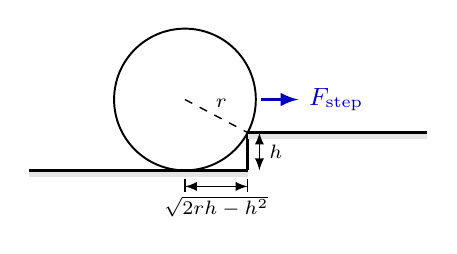
\begin{tikzpicture}[scale=6, >=latex]

  %% ---- Parameters ----
  \pgfmathsetmacro{\rr}{0.15}
  \pgfmathsetmacro{\hh}{0.08}

  %% ---- Derived ----
  \pgfmathsetmacro{\cx}{sqrt(2*\rr*\hh - \hh*\hh)}

  %% ---- Lower ground (left) ----
  \fill[gray!20] ({-\cx-\rr-0.18}, {-0.013}) rectangle (0, 0);
  \draw[line width=1.0pt] ({-\cx-\rr-0.18}, 0) -- (0, 0);

  %% ---- Step vertical face ----
  \draw[line width=1.0pt] (0, 0) -- (0, {\hh});

  %% ---- Upper ground (right) ----
  \fill[gray!20] (0, {\hh-0.013}) rectangle (0.38, {\hh});
  \draw[line width=1.0pt] (0, {\hh}) -- (0.38, {\hh});

  %% ---- Wheel ----
  \draw[line width=0.7pt] ({-\cx}, {\rr}) circle (\rr);

  %% ---- r: dashed line, label shifted above-left clear of circle stroke ----
  \draw[dashed, line width=0.5pt]
    ({-\cx}, {\rr}) -- (0, {\hh});
  \node[font=\scriptsize] at ({-\cx*0.42}, {\rr + (\hh-\rr)*0.42 + 0.022})
    {$r$};

  %% ---- h: vertical arrow right of step face ----
  \draw[latex-latex, line width=0.5pt]
    (0.025, 0) -- (0.025, {\hh})
    node[midway, right, font=\scriptsize] {$h$};

  %% ---- sqrt(2rh-h^2): horizontal arrow below lower ground ----
  \draw[latex-latex, line width=0.5pt]
    ({-\cx}, {-0.034}) -- (0, {-0.034})
    node[midway, below, font=\scriptsize] {$\sqrt{2rh - h^2}$};
  \draw[line width=0.4pt] ({-\cx}, {-0.018}) -- ({-\cx}, {-0.046});
  \draw[line width=0.4pt] (0,      {-0.018}) -- (0,      {-0.046});

  %% ---- F_step arrow ----
  \draw[->, line width=1.2pt, blue!75!black]
    ({-\cx+\rr+0.012}, {\rr})
    -- ({-\cx+\rr+0.09}, {\rr})
    node[right, font=\small\bfseries] {$F_{\mathrm{step}}$};

\end{tikzpicture}
\caption{Step-climbing geometry with obstacle height $h$ and wheel radius $r$.}
\label{fig:step_geom}
<<<<<<< des/2_1_3_wheel_design
\vspace{-0.5\baselineskip}
\end{wrapfigure}

Drive motor selection was based on two parallel analyses.
First, a traction model accounting for rover mass, rolling
resistance of Mars~yard terrain, and a \ang{15} slope yields
a required wheel torque of approximately \SI{12}{\newton\metre}
per wheel at \SI{1}{\metre\per\second} with \SI{1}{\second}
acceleration time. Applying a safety factor of $k_s = 1.5$ and
assuming drivetrain efficiency of $\eta = 0.8$ gives a rated
motor requirement of approximately \SI{23.8}{\newton\metre}.
Second, a step-climbing torque analysis was performed, relating
required wheel torque to obstacle height for a wheel radius of
\SI{150}{\milli\metre}; this sets an upper bound of approximately
\SI{40}{\newton\metre} for the maximum obstacle height of
$h^* \approx \SI{127}{\milli\metre}$ (${\approx}\,85\%$ of wheel
radius). Based on these results, the \mbox{DM-J10010L-2EC} hub
motor was selected, providing \SI{40}{\newton\metre} nominal and
\SI{120}{\newton\metre} peak torque at \SI{48}{\volt} ---
satisfying both the traction and obstacle-climbing requirements
with adequate margin. To simplify logistics and electronics
development, the same motor model is used for wheel drive and the shoulder joints of the
manipulator arm.
=======
\end{subfigure}\hfill
\begin{subfigure}[t]{0.49\linewidth}
\centering
\begin{tikzpicture}[scale=0.82, >=Stealth]
  % Slope and horizontal reference
  \draw[gray!60, dashed] (-0.4,0) -- (5.0,0);
  \draw[line width=1.0pt] (0,0) -- ({4.8*cos(15)},{4.8*sin(15)});

  % Wheel geometry on slope
  \pgfmathsetmacro{\rw}{0.55}
  \coordinate (P) at ({2.0*cos(15)},{2.0*sin(15)});
  \coordinate (C) at ({2.0*cos(15)-\rw*sin(15)},{2.0*sin(15)+\rw*cos(15)});
  \draw[line width=0.9pt] (C) circle (\rw);
  \fill (C) circle (1.1pt);

  % Velocity vector uphill (Formula 1 case)
  \draw[->, line width=1.1pt, blue!75!black]
    (C) -- ++({1.15*cos(15)},{1.15*sin(15)})
    node[above right, font=\scriptsize] {$v=\SI{1}{\metre\per\second}$};

  % Weight vector
  \draw[->, line width=0.9pt, red!70!black]
    (C) -- ++(0,-1.0)
    node[right, font=\scriptsize] {$mg$};

  % Slope angle label
  \draw[->, line width=0.6pt] (0.95,0) arc[start angle=0, end angle=15, radius=0.95];
  \node[font=\scriptsize] at (0.82,-0.12) {$\alpha=\ang{15}$};
\end{tikzpicture}
\caption{Uphill case from Formula~1: \ang{15} slope and $v=\SI{1}{\metre\per\second}$.}
\label{fig:uphill_motion_formula1}
\end{subfigure}
\end{minipage}

\caption{Locomotion load cases used for drivetrain sizing.}
\label{fig:locomotion_load_cases}
\end{figure}

Drivetrain torque sizing is based on two governing load cases: uphill traction and step climbing.

All calculations in this subsection are approximate engineering estimates used for system-level sizing, with conservative margin applied in final actuator requirements.

\begin{itemize}[leftmargin=1.2em, itemsep=0.2em, topsep=0.3em]
  \item \textbf{Traction case (\ang{15} slope):} estimated wheel torque
  $\tau_\mathrm{wheel}\approx\SI{12.7}{\newton\metre}$ at
  $v=\SI{1}{\metre\per\second}$ and
  $a=\SI{1}{\metre\per\second\squared}$.

  \item \textbf{Rated motor requirement:} with safety factor
  $k_s=1.5$ and drivetrain efficiency $\eta=0.8$,
  $\tau_\mathrm{rated}\approx\SI{23.8}{\newton\metre}$.

  \item \textbf{Step-climbing case:} for wheel radius
  $r=\SI{150}{\milli\metre}$, the nominal torque limit
  $\SI{40}{\newton\metre}$ corresponds to
  $h^*\approx\SI{127}{\milli\metre}\;(\approx0.85r)$.

  \item \textbf{Motor selection:} \textit{Drive Motor},
  with \SI{40}{\newton\metre} nominal and
  \SI{120}{\newton\metre} peak capability at 48~V,
  covering both load cases with margin.

  \item \textbf{Standardization:} the same motor class is used for
  wheel drive, steering rotation, and manipulator shoulder joints.
\end{itemize}
>>>>>>> main


\begin{table}[h!]
\centering
\caption{Drive motor torque requirements (\(r = \SI{150}{\milli\metre}\), \(m = \SI{75}{\kilo\gram}\), \(N{=}4\) wheels)}
\label{tab:motor_torque}
\setlength{\tabcolsep}{8pt}
\begin{tabular}{@{}llll@{}}
\toprule
\textbf{Load case} & \textbf{Expression} & \textbf{Value} & \textbf{Note} \\
\midrule
\multicolumn{4}{@{}l}{\textit{Traction model}} \\[2pt]
Rolling resistance
  & $F_\mathrm{roll} = C_{rr}\,mg$
  & \SI{73.6}{\newton}
  & $C_{rr}=0.10$ \\
Grade force
  & $F_\mathrm{grade} = mg\sin\alpha$
  & \SI{190.4}{\newton}
  & $\alpha=\ang{15}$ \\
Acceleration force
  & $F_\mathrm{acc} = ma$
  & \SI{75.0}{\newton}
  & $a=\SI{1}{\metre\per\second\squared}$ \\
Total traction force
  & $F_\mathrm{tot} = F_\mathrm{acc}+F_\mathrm{roll}+F_\mathrm{grade}$
  & \SI{339.0}{\newton}
  & \\
Wheel torque
  & $\tau_\mathrm{wheel} = F_\mathrm{tot}\,r/N$
  & \SI{12.7}{\newton\metre}
  & per wheel \\
\textbf{Rated requirement}
  & $\tau_\mathrm{rated} = \tau_\mathrm{wheel}\,k_s/\eta$
  & \textbf{\SI{23.8}{\newton\metre}}
  & $k_s{=}1.5,\;\eta{=}0.8$ \\[4pt]
\multicolumn{4}{@{}l}{\textit{Step-climbing model}} \\[2pt]
Front wheel load
  & $W_\mathrm{front} = mg/N$
  & \SI{183.9}{\newton}
  & 50\,\% front share, 2 wheels \\
Step torque
  & $\tau_\mathrm{step}(h)
    = W_\mathrm{front}\,r\,\dfrac{\sqrt{2rh-h^2}}{r-h}$
  & ---
  & \\
Max obstacle (nominal)
  & $\tau_\mathrm{step}(h^*) = \SI{40}{\newton\metre}$
  & $h^* \approx \SI{127}{\milli\metre}$
  & $0.85\,r$ \\
Max obstacle (peak)
  & $\tau_\mathrm{step}(h^{**}) = \SI{120}{\newton\metre}$
  & $h^{**} \approx \SI{148}{\milli\metre}$
  & $0.99\,r$ \\
\bottomrule
\end{tabular}
\end{table}

\paragraph{Wheel Design}
\label{par:wheel_design}
% Tiny contract
% Teams: Suspension
% Requirements: REQ-DES-130 REQ-FUN-020
% Status: [in-progress]

The rover wheels are manufactured as single-piece TPU components to reduce assembly 
complexity and provide controlled elastic compliance on irregular terrain. A chevron-type 
tread is used to improve longitudinal traction and reduce lateral slip on loose soil and 
mixed rocky surfaces typical of the ERC Mars Yard.

To reduce unsprung mass, the wheel body uses a perforated web pattern. The geometry 
was verified by finite-element analysis under a maximum wheel load of \SI{45}{\kilo\gram}, 
with the design target of limiting peak deformation to \SI{5}{\milli\metre}. The current 
wheel revision satisfies this deformation criterion and is used as the baseline for mass, 
traction, and endurance tests.

\begin{figure}[H]
\centering
\begin{minipage}[t]{0.48\linewidth}
	\centering
	\fbox{\parbox[c][4.0cm][c]{0.92\linewidth}{\centering
	Wheel design image\\placeholder}}
\end{minipage}\hfill
\begin{minipage}[t]{0.48\linewidth}
	\centering
	\fbox{\parbox[c][4.0cm][c]{0.92\linewidth}{\centering
	FEA simulation image\\placeholder}}
\end{minipage}
\caption{Wheel design and FEA simulations.}
\label{fig:wheel_and_fea_placeholders}
\end{figure}



\paragraph{Turning Radius and Steering Kinematics}
\label{par:turning_radius_steering_kinematics}
% Tiny contract
% Teams: [team-name]
% Requirements: [REQ-*]
% Status: [draft|in-progress|done]

% Placeholder content for sections/design/2/2_1/2_1_3_turning_radius_steering_kinematics.tex

Each wheel can rotate independently through 360° under software control. The angular position of each wheel is determined by an absolute encoder integrated into the steering mechanism. Wheels can be positioned such that the rover rotates about its own axis, achieving a minimum turning radius of approximately 700 mm.

Detailed kinematic derivations, including the formal Ackermann steering model and control constraints, will be added in a later revision of this subsection.

\begin{figure}[htbp]
	\centering
	\fbox{\parbox[c][5.0cm][c]{0.9\linewidth}{\centering
		Placeholder for Ackermann kinematics diagram of the rover\\
		(top-view geometry, wheel angles, and turning center)
	}}
	\caption{Ackermann steering kinematics of the rover (placeholder)}
	\label{fig:rover_ackermann_kinematics_placeholder}
\end{figure}

\begin{figure}[htbp]
	\centering
	\fbox{\parbox[c][5.0cm][c]{0.9\linewidth}{\centering
		Placeholder for lateral (crab) rover motion image\\
		(all wheels rotated for side movement)
	}}
	\caption{Rover lateral motion with 360-degree wheel steering (placeholder)}
	\label{fig:rover_crab_motion_placeholder}
\end{figure}



\paragraph{Manipulator Configuration and Kinematics}
\label{par:manipulator_configuration_kinematics}
\input{sections/design/2_rover_design_description/2_1_mechanical_design/2_1_5_manipulator_configuration_kinematics}

\paragraph{Joint Design and Actuators}
\label{par:joint_design_actuators}
\input{sections/design/2_rover_design_description/2_1_mechanical_design/2_1_6_joint_design_actuators}

\paragraph{End-Effector Design}
\label{par:end_effector_design}
% Tiny contract
% Teams: arm
% Requirements: REQ-GEN-090, REQ-FUN-100, REQ-DES-140
% Status: done

\subsubsection{End-Effector Design}
\label{subsubsec:end_effector_design}

The rover employs a parallel-jaw gripper mechanism for maintenance operations and sample collection tasks. The design features a dual-linkage symmetric four-bar configuration maintaining parallel finger pad orientation throughout the \qty{105}{\milli\metre} maximum opening range, ensuring uniform pressure distribution and consistent tool center point (TCP) alignment (\autoref{fig:gripper_assembly}).

\begin{figure}[H]
    \centering
    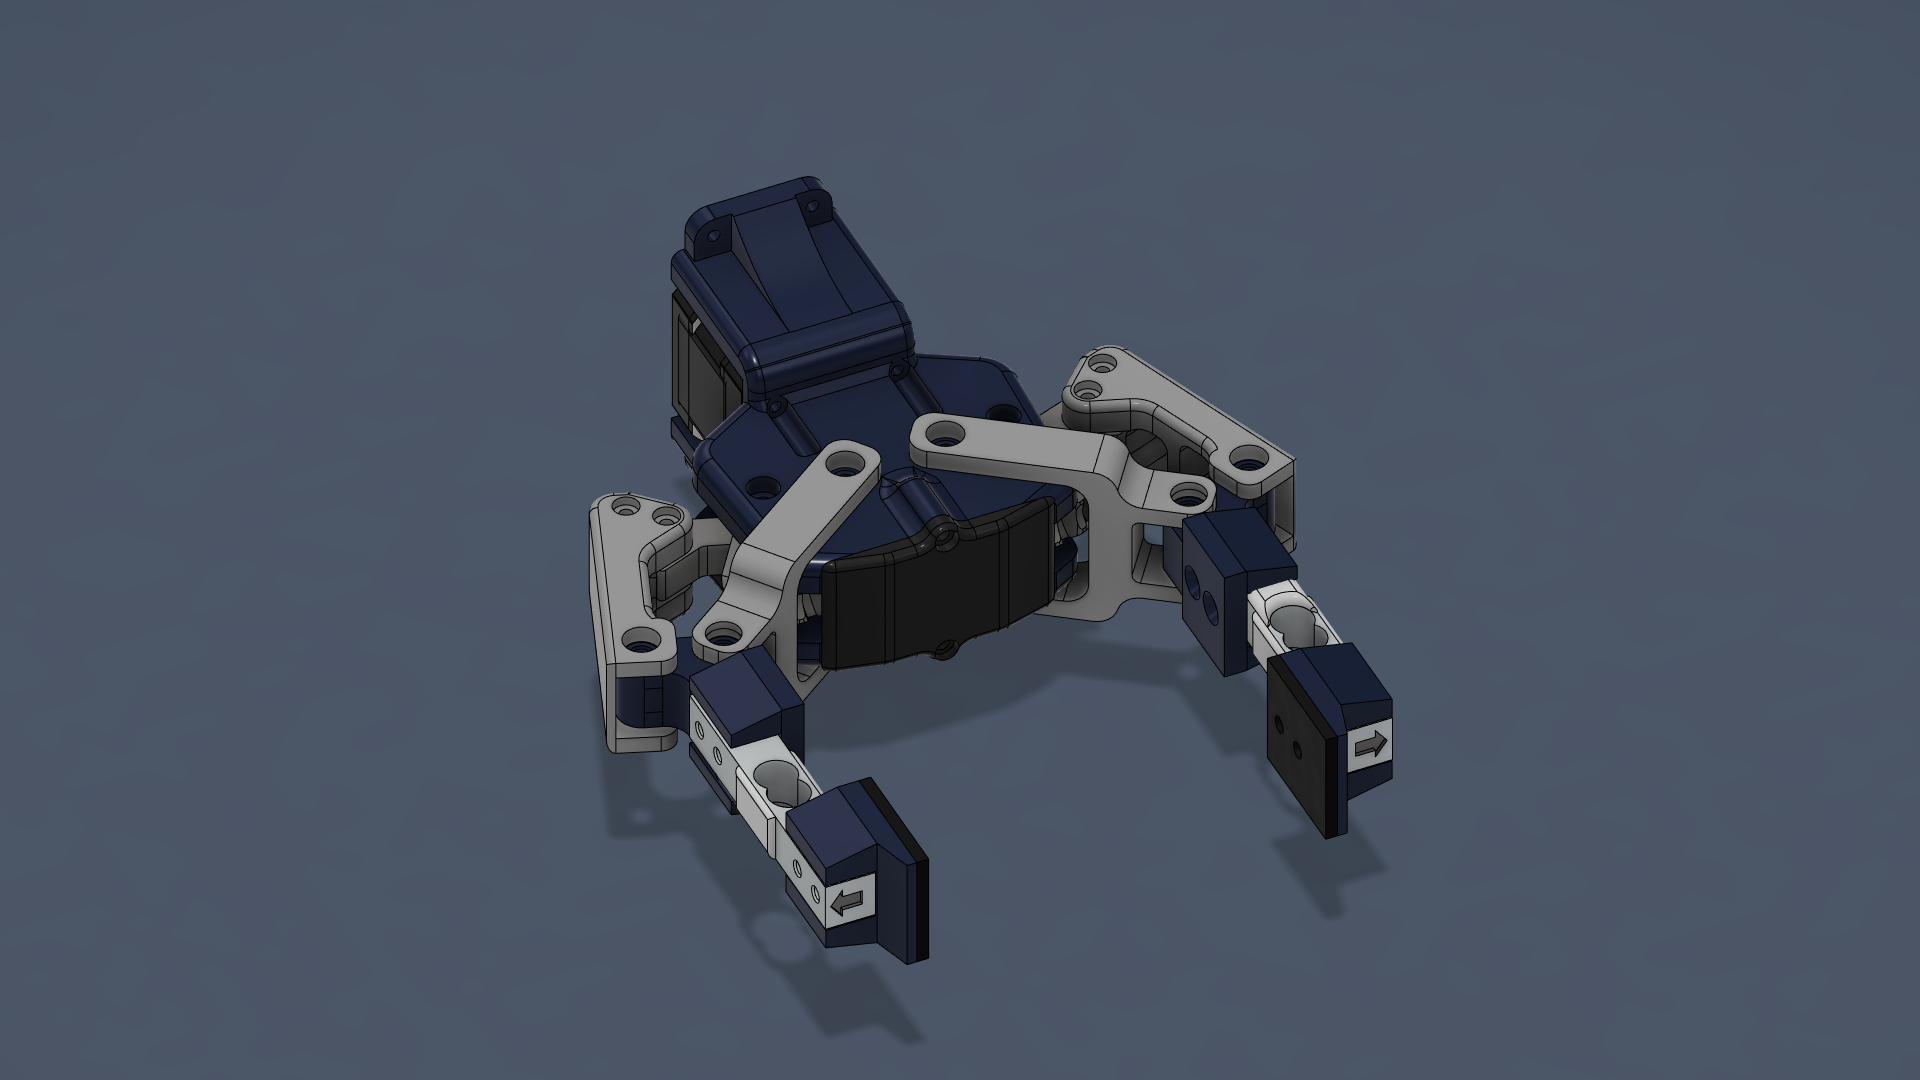
\includegraphics[width=0.7\textwidth]{teams/arm/figures/gripper_assembly.png}
    \caption{Gripper assembly showing dual-linkage mechanism and finger geometry}
    \label{fig:gripper_assembly}
\end{figure}

\paragraph{Kinematic Architecture}
The symmetrically mirrored four-bar linkage arrangement provides mechanical advantage through two aluminum linkages per finger, pinned at discrete pivot points to form a robust mechanical loop. This configuration constrains gripping surfaces to remain parallel during actuation, preventing object rotation and ensuring repeatable force vectors. Symmetric design about both longitudinal and lateral axes maintains grasp center alignment with the TCP for precise manipulation coupled with robotic arm kinematics (\autoref{subsubsec:manipulator_configuration_kinematics}).

\paragraph{Actuation and Force Sensing}
NEMA17 stepper motor actuation provides sufficient torque with inherent overload protection through step-skipping behavior, preventing mechanical damage during constrained motion. Integrated Force-sensitive Hall-effect Dual-Axis (FHDA) load sensors enable closed-loop force control, modulating grip strength based on object compliance to prevent crushing fragile components while ensuring secure retention during manipulation and transport.

\paragraph{Gripper Geometry and Contact Surfaces}
Active gripping surfaces measuring \numproduct{30 x 32}~mm feature molded rubber pads increasing friction while providing mechanical damping. Compliant pads accommodate non-planar geometries and absorb impact forces during tasks such as switch rotation. Fingertip geometry narrows to \qty{10}{\milli\metre} total width for precise engagement with circuit breaker switches (\qtyrange{10}{15}{\milli\metre} width) and small-profile panel targets. Overall dimensions when fully opened are \numproduct{180 x 200 x 80}~mm (W$\times$L$\times$H).

\paragraph{Panel Operation Capabilities}
Parallel-jaw configuration with force feedback enables controlled pressing motions on panel buttons with programmable force profiles. Narrow fingertip geometry permits switch engagement in densely populated control panels. Rubber pad compliance allows rotational manipulation of cylindrical knobs and toggle switches through friction coupling. Combined position control and force sensing support typing, button pressing, and connector insertion/extraction operations on maintenance panels.

\paragraph{Probe Collection}
The gripper accommodates cylindrical aluminum probes (\qty{30}{\milli\metre} diameter, \qty{200}{\milli\metre} height) through its \qty{105}{\milli\metre} maximum jaw opening. Parallel-jaw mechanism distributes gripping forces evenly around probe circumference, preventing structural deformation. Rubber pads provide anti-slip characteristics for secure retention during arm motion and probe extraction from ground insertion points. Force sensing enables adaptive grip pressure accounting for surface conditions and extraction resistance.

\paragraph{Mechanical Interface}
The gripper base features standardized mounting geometry for attachment to the robotic arm's quick-change end-effector mount, enabling rapid tool exchange. Mechanical and electrical interfaces ensure reliable coupling under field conditions with minimal alignment sensitivity.


\paragraph{Sample Storage and Weighing System}
\label{par:sample_storage_weighing_system}
\input{sections/design/2_rover_design_description/2_1_mechanical_design/2_1_8_sample_storage_weighing_system}

\paragraph{Drill System Implementation}
\label{par:drill_system_implementation}
\input{sections/design/2_rover_design_description/2_1_mechanical_design/2_1_9_drill_system_implementation}

\subsubsection{Electrical Power Subsystem}
\label{subsubsec:electrical_power_subsystem}

\paragraph{Battery Configuration and Hot-Swap Design}
\label{par:battery_configuration_hotswap_design}
\input{sections/design/2_rover_design_description/2_2_electrical_power_subsystem/2_2_1_battery_configuration_hotswap_design}

\paragraph{Power Distribution and Regulation}
\label{par:power_distribution_regulation}
\input{sections/design/2_rover_design_description/2_2_electrical_power_subsystem/2_2_2_power_distribution_regulation}

\subsubsection{Communication Subsystem}
\label{subsubsec:communication_subsystem}

\paragraph{Communication Architecture Overview}
\label{par:communication_architecture_overview}
\input{sections/design/2_rover_design_description/2_3_communication_subsystem/2_3_1_communication_architecture_overview}

\paragraph{Frequency Plan}
\label{par:frequency_plan}
\input{sections/design/2_rover_design_description/2_3_communication_subsystem/2_3_2_frequency_plan}

\paragraph{Antenna Design and Placement}
\label{par:antenna_design_placement}
\input{sections/design/2_rover_design_description/2_3_communication_subsystem/2_3_3_antenna_design_placement}

\paragraph{Interference Mitigation}
\label{par:interference_mitigation}
\input{sections/design/2_rover_design_description/2_3_communication_subsystem/2_3_4_interference_mitigation}

\paragraph{Link Performance Analysis}
\label{par:link_performance_analysis}
\input{sections/design/2_rover_design_description/2_3_communication_subsystem/2_3_5_link_performance_analysis}

\paragraph{Bandwidth Management}
\label{par:bandwidth_management}
\input{sections/design/2_rover_design_description/2_3_communication_subsystem/2_3_6_bandwidth_management}

\paragraph{Communication Redundancy}
\label{par:communication_redundancy}
\input{sections/design/2_rover_design_description/2_3_communication_subsystem/2_3_7_communication_redundancy}

\subsubsection{On-Board Sensor and Imaging Systems}
\label{subsubsec:onboard_sensor_imaging_systems}

\paragraph{Navigation Sensor Suite\reqtags{FUN-220 | FUN-240 | ENV-040}}
\label{par:navigation_sensor_suite}
% Tiny contract
% Teams: Navigation
% Requirements: REQ-FUN-220, REQ-FUN-240, REQ-ENV-040
% Status: done

The navigation sensor suite provides near-\ang{360} perception for simultaneous state estimation and collision avoidance.

\begin{itemize}
	\item \textbf{Front stereo vision (ZED 2i):} RGB imagery and depth at \numproduct{1280 x 720} and \qty{60}{\fps}. Field of view: \ang{110}~$\times$~\ang{70} (H$\times$V). Effective depth range: \qtyrange{0.3}{20}{\metre}. The integrated 6-axis IMU (\qty{400}{\hertz}) and magnetometer support inertial state estimation.

	\item \textbf{Top LiDAR (RPLIDAR S2):} \ang{360} 2D scanning with \ang{0.12} angular resolution at \qty{10}{\hertz}. Reliable obstacle detection up to \qty{10}{\metre} across varying lighting and reflectivity conditions.

	\item \textbf{Side and rear close-range coverage (3\,$\times$ Maix Sense A010 ToF):} Sensors mounted on the left flank, right flank, and rear provide \ang{210} non-forward coverage. Each sensor outputs a \numproduct{100 x 100} depth map at up to \qty{20}{\fps} with \ang{70}~$\times$~\ang{60} (H$\times$V) FoV and an effective range of \qtyrange{0.2}{2.5}{\metre}. Performance may degrade under direct bright sunlight.

	\item \textbf{Wheel odometry:} Swerve drive modules use 14-bit single-turn absolute magnetic encoders, providing immediate and precise angular feedback for drive and steering shafts.
\end{itemize}

The ZED 2i, RPLIDAR S2, and encoders provide input to state estimation and localization (\autoref{par:state_estimation_localization}), while all vision and ranging sensors support collision avoidance (\autoref{par:autonomous_navigation_collision_avoidance}).

\paragraph{Science Sensor Suite}
\label{par:science_sensor_suite}
\input{sections/design/2_rover_design_description/2_4_onboard_sensor_imaging_systems/2_4_2_science_sensor_suite}

\paragraph{Rover Camera Suite}
\label{par:rover_camera_suite}
% Tiny contract
% Teams: Science Team, Ground Station Team, Arm Team
% Requirements: REQ-FUN-170, REQ-GEN-080, REQ-FUN-130
% Status: in-progress

% Placeholder content for sections/design/2/2_4/2_4_3_rover_camera_suite.tex

An Arducam AR0234 color global shutter USB 3.0 camera is mounted \qty{10}{\centi\metre} above the gripper, aligned parallel to its orientation to support object recognition and pose estimation. The global shutter sensor ensures blur-free imaging during dynamic arm movements. The module utilizes an M12 manual-focus lens ($f = \qty{3.6}{\milli\metre}$) delivering an \ang{82}~$\times$~\ang{66} (H$\times$V) FoV with low ($\sim$\qty{3}{\percent}) distortion.

% TODO: Specify illumination module (e.g., LED floodlight/COB), beam angle (>\ang{120}), maybe power draw, and maybe PWM control
Integrated wide-angle illumination provides consistent, shadow-free visibility of the front working area during maintenance and liquid sampling operations.


% TODO: paragraphs for Science Team and Ground Station Team


\subsubsection{Software Architecture}
\label{subsubsec:software_architecture}

\paragraph{Software System Overview}
\label{par:software_system_overview}
\input{sections/design/2_rover_design_description/2_5_software_architecture/2_5_1_software_system_overview}

\paragraph{State Estimation and Localization}
\label{par:state_estimation_localization}
\input{sections/design/2_rover_design_description/2_5_software_architecture/2_5_2_state_estimation_localization}

\paragraph{Autonomous Navigation and Collision Avoidance}
\label{par:autonomous_navigation_collision_avoidance}
% Tiny contract
% Teams: Navigation
% Requirements: REQ-OPS-050, REQ-FUN-060, REQ-FUN-240
% Status: done

The navigation subsystem performs autonomous path planning, trajectory tracking, and collision avoidance. After receiving a goal pose or waypoint sequence, the rover executes motion in a closed loop: sensor updates (\autoref{par:navigation_sensor_suite}), costmap update, global planning, local trajectory tracking, and command execution. The same stack is used for traversal and task positioning, while manipulation is handled separately (\autoref{par:arm_kinematics_motion_planning}).

Global planning uses NavFn (Dijkstra) over a \qty{0.05}{\metre} resolution 2D costmap. Local motion tracks the global path while reacting in real time to terrain changes and newly detected obstacles. Collision avoidance, including other rovers (REQ-FUN-240), is enforced through obstacle detection and safety-margin inflation.

The costmap integrates depth and range sensing into voxel, obstacle, and inflation layers at \qty{0.05}{\metre} resolution. Obstacles include occupied cells, terrain protrusions above \qty{0.15}{\metre}, depressions deeper than \qty{0.10}{\metre}, and cells with cost $\geq 253$. Traversability is estimated from terrain geometry, with safe regions defined by cost thresholds.

If the path becomes obstructed, the navigation state machine (Figure~\ref{fig:navigation_combined}) performs local recovery, triggers global replanning if needed, or executes a fail-safe stop if no safe trajectory is found within a timeout.
\begin{figure}[H]
  \centering

  \begin{minipage}{0.49\linewidth}
    \centering
    \resizebox{\linewidth}{!}{% Nav2 dataflow diagram - corrected final version
% Requires in preamble.tex:
% \usetikzlibrary{arrows.meta,positioning,calc,backgrounds,fit}

\tikzset{
  blk/.style={
    rectangle, draw=black, fill=white, text=black, line width=0.5pt,
    minimum width=4.2cm, minimum height=0.95cm,
    align=center, font=\small,
    inner ysep=2pt
  },
  arr/.style={-{Stealth[length=2.5pt]}, line width=0.5pt, draw=black},
}

\begin{tikzpicture}[node distance=1.45cm and 2.55cm]

  %% === SENSORS COLUMN ===
  \node[blk] (stereo) {StereoLabs ZED 2i\\[-1pt]{\scriptsize USB 3.0 - 110\textdegree$\times$70\textdegree{} FOV}};
  \node[blk] (tof) [below=of stereo] {ToF Cameras $\times$3\\[-1pt]{\scriptsize MaixSense A010 - I2C}};
  \node[blk] (lidar) [below=of tof] {RPLIDAR-S2\\[-1pt]{\scriptsize UART - 360\textdegree{} - 10\,Hz}};

  %% === COSTMAP COLUMN ===
  \node[blk] (voxel) [right=of stereo] {Voxel Layer\\[-1pt]{\scriptsize 3D grid - 0.05\,m resolution}};
  \node[blk] (obstacle) [below=of voxel] {Obstacle Layer\\[-1pt]{\scriptsize 2D projection}};
  \node[blk] (inflation) [below=of obstacle] {Inflation Layer\\[-1pt]{\scriptsize radius 0.15\,m}};

  %% === NAV2 COLUMN ===
  \node[blk] (global) [right=3.45cm of voxel] {NavFn Planner\\[-1pt]{\scriptsize Dijkstra - $<500$\,ms}};
  \node[blk] (local) [below=of global] {DWB Controller\\[-1pt]{\scriptsize 20\,Hz - $(v,\omega)$}};
  \node[blk] (cmdvel) [below=of local] {Motor Controllers};

  %% === SENSOR INPUTS ===
  \draw[arr] (stereo.east) -- ++(0.80,0) |- (voxel.west);
  \node[font=\scriptsize] at ($(stereo.east)!0.56!(voxel.west)+(0,0.28)$) {Depth};

  \draw[arr] (tof.east) -- ++(0.80,0) |- (voxel.west);
  \node[font=\scriptsize] at ($(tof.east)!0.56!(voxel.west)+(0,0.75)$) {Range};

  \draw[arr] (lidar.east) -- ++(1.90,0) |- (obstacle.west);
  \node[font=\scriptsize] at ($(lidar.east)+(1.10,0.28)$) {LaserScan};

  %% === COSTMAP PIPELINE ===
  \draw[arr] (voxel.south) -- (obstacle.north)
    node[midway, right, font=\scriptsize] {voxels};

  \draw[arr] (obstacle.south) -- (inflation.north)
    node[midway, right, font=\scriptsize] {obstacles};

  %% === COSTMAP -> GLOBAL PLANNER ===
  \coordinate (cgA) at ($(inflation.east)+(0.60,0)$);
  \coordinate (cgB) at ($(cgA |- global.west)$);
  \draw[arr] (inflation.east) -- (cgA) -- (cgB) -- (global.west);
  \node[font=\scriptsize, above] at ($(cgB)!0.5!(global.west)+(0.00,0.12)$) {Costmap};

  %% === COSTMAP -> LOCAL CONTROLLER ===
  \coordinate (clA) at ($(inflation.east)+(1.05,0)$);
  \coordinate (clB) at ($(clA |- local.west)$);
  \draw[arr] (inflation.east) -- (clA) -- (clB) -- (local.west);
  \node[font=\scriptsize, above] at ($(clB)!0.5!(local.west)+(-0.25,0.12)$) {Local costmap};

  %% === GLOBAL PLAN -> LOCAL CONTROLLER ===
  \draw[arr] (global.south) -- (local.north);
  \node[font=\scriptsize, right, align=left]
    at ($(global.south)!0.5!(local.north)+(0.16,0.00)$)
    {\texttt{nav\_msgs/}\\\texttt{Path}};

  %% === OUTPUT ===
  \draw[arr] (local.south) -- (cmdvel.north);
  \node[font=\scriptsize, right, align=left]
    at ($(local.south)!0.56!(cmdvel.north)+(0.16,0.00)$)
    {\texttt{geometry\_msgs/}\\\texttt{Twist}};

  %% === COLUMN LABELS ===
  \node[font=\small\bfseries, above=0.55cm of stereo] {SENSOR SUITE};
  \node[font=\small\bfseries, above=0.55cm of voxel] {COSTMAP};
  \node[font=\small\bfseries, above=0.55cm of global] {NAV2 STACK};

  %% === SECTION FRAMES ===
  \begin{scope}[on background layer]
    \node[
      draw=black, fill=black!5, dashed, line width=0.8pt,
      inner sep=8pt, rounded corners=3pt,
      fit=(stereo)(lidar)
    ] {};

    \node[
      draw=black, fill=black!5, dashed, line width=0.8pt,
      inner sep=8pt, rounded corners=3pt,
      fit=(voxel)(inflation)
    ] {};

    \node[
      draw=ercblue, fill=ercblue!5, dashed, line width=0.8pt,
      inner sep=8pt, rounded corners=3pt,
      fit=(global)(cmdvel)
    ] {};
  \end{scope}

\end{tikzpicture}}
  \end{minipage}
  \hfill
  \begin{minipage}{0.49\linewidth}
    \centering
    \resizebox{\linewidth}{!}{% Navigation state machine - corrected with larger label spacing
% Requires:
% \usetikzlibrary{arrows.meta,positioning,calc}

\tikzset{
  blk/.style={
    rectangle, draw=black, fill=white, line width=0.5pt,
    minimum width=3.8cm, minimum height=0.9cm,
    align=center, font=\small
  },
  arr/.style={-{Stealth[length=2.5pt]}, line width=0.5pt, draw=black},
  dlink/.style={-{Stealth[length=2.5pt]}, line width=0.5pt, dashed, draw=black},
}

\begin{tikzpicture}[node distance=1.9cm and 2.5cm]

  %% === STATES - Row 1 ===
  \node[blk] (idle) {IDLE\\{\scriptsize waiting for goal}};
  \node[blk] (compute) [right=3.0cm of idle]
    {COMPUTE PATH\\{\scriptsize NavFn - Dijkstra}};
  \node[blk] (drive) [right=of compute]
    {TRACK TRAJECTORY\\{\scriptsize DWB - 20\,Hz}};

  %% === STATES - Row 2 ===
  \node[blk] (waypoint) [below=of idle]
    {WAYPOINT REACHED\\{\scriptsize tolerance 0.75\,m}};
  \node[blk] (replan) [below=of compute]
    {REPLAN\\{\scriptsize NavFn recompute}};
  \node[blk] (evasion) [below=of drive]
    {LOCAL EVASION\\{\scriptsize local recovery attempt}};

  %% === FAIL-SAFE STATE ===
  \node[blk] (stop) [below=of replan]
    {FAIL-SAFE STOP\\{\scriptsize no safe trajectory}};

  %% === MAIN FLOW ===
  \draw[arr] (idle.east) -- (compute.west)
    node[midway, above=3pt, font=\scriptsize] {goal pose received};

  \draw[arr] (compute.east) -- (drive.west)
    node[midway, above, font=\scriptsize] {path valid};

  %% === TRACK -> LOCAL EVASION ===
  \draw[arr] (drive.south) -- (evasion.north);
  \node[font=\scriptsize, left] at ($(drive.south)!0.55!(evasion.north)+(-0.35,0)$)
    {path obstructed};

  %% === LOCAL EVASION -> REPLAN ===
  \draw[arr] (evasion.west) -- (replan.east);
  \node[font=\scriptsize, above] at ($(evasion.west)!0.5!(replan.east)+(0,0.12)$)
    {local evasion failed};

  %% === REPLAN -> COMPUTE PATH ===
  \draw[arr] (replan.north) -- (compute.south)
    node[midway, right, font=\scriptsize] {replan request};

  %% === HELPER COORDINATES ===
  \coordinate (lefttop) at ([xshift=-0.95cm]idle.west);
  \coordinate (leftbot) at ([xshift=-0.95cm]waypoint.west);
  \coordinate (topline) at ([yshift=1.00cm]drive.north);

  %% === TRACK -> WAYPOINT REACHED ===
  \draw[arr]
    (drive.north) -- (topline)
    -| (lefttop)
    -- (leftbot)
    -- (waypoint.west);

  \node[font=\scriptsize, above]
    at ($(topline)+(-4.9cm,0)$) {position error $< 0.75\,m$};

  %% === WAYPOINT REACHED -> IDLE ===
  \draw[arr]
    ([xshift=0.45cm]waypoint.north) -- ([xshift=0.45cm]idle.south);

  \node[font=\scriptsize, right]
    at ($([xshift=0.45cm]waypoint.north)!0.5!([xshift=0.45cm]idle.south)$)
    {next waypoint};

  %% === REPLAN -> FAIL-SAFE STOP ===
  \draw[dlink] (replan.south) -- (stop.north)
    node[midway, right, font=\scriptsize] {replan timeout 10\,s};

  %% === LOCAL EVASION -> TRACK TRAJECTORY ===
  \coordinate (pc1) at ([xshift=0.70cm]evasion.east);
  \coordinate (pc2) at ([xshift=0.70cm,yshift=1.75cm]evasion.east);

  \draw[dlink] (evasion.east) -- (pc1) -- (pc2) -- (drive.east);

  \node[font=\scriptsize, right]
    at ($(pc1)!0.52!(pc2)+(0.22,0)$) {local path clear};

\end{tikzpicture}}
  \end{minipage}

  \caption{Navigation overview: state machine and data flow}
  \label{fig:navigation_combined}
\end{figure}

\paragraph{Arm Kinematics and Motion Planning}
\label{par:arm_kinematics_motion_planning}
% Tiny contract
% Teams: [team-name]
% Requirements: [REQ-*]
% Status: [draft|in-progress|done]

% Placeholder content for sections/design/2/2_5/2_5_4_arm_kinematics_motion_planning.tex


\subsection{Manipulator Motion Control}

\subsubsection{Manipulator Control Software Stack}
The manipulator is controlled using a \textbf{ROS 2-based stack} in which \textbf{URDF/SRDF} define the robot model, \textbf{MoveIt 2} handles motion planning, \textbf{KDL} provides kinematics, \textbf{OMPL} generates trajectories, and \textbf{ros2\_control} sends commands to the real actuators. \textbf{Custom ROS 2 nodes} implement the application logic, while the \textbf{CV module} provides scene and target object data to MoveIt.

\subsubsection{Kinematic Model Representation}
The manipulator kinematic model is defined as an \textbf{XML-based description using URDF/Xacro and SRDF}, including links, joints, geometry, motion axes, limits, the base frame \texttt{base\_link}, and the tool frame \texttt{tool0} or \texttt{end\_effector}. This model is used for FK, IK, collision checking, and motion planning.

\subsubsection{Forward Kinematics}
\textbf{Forward kinematics (FK)} is handled by \textbf{MoveIt 2} using \textbf{KDL} as the underlying solver. It takes current joint values as input and computes the position and orientation of the end effector.

\subsubsection{Inverse Kinematics}
\textbf{Inverse kinematics (IK)} is performed by \textbf{KDL within MoveIt 2}. Given a target end-effector pose, it computes a valid joint configuration consistent with the manipulator geometry and motion limits.

\subsubsection{FK/IK Configuration for the Manipulator Geometry}
FK and IK are configured through the \textbf{URDF/Xacro model}, which defines the actual joint order, joint types, rotation axes, zero positions, joint limits, link offsets, and the \textbf{TCP} location relative to the end effector. This binds the kinematic solver to the real manipulator geometry.

\subsubsection{Motion Constraints}
Motion constraints are defined at several levels: \textbf{URDF} specifies joint types and limits, \textbf{SRDF/MoveIt} defines planning groups and logical constraints, and trajectory planning additionally considers workspace limits, self-collision, collision objects, and motion safety constraints.

\subsubsection{Trajectory Generation}
Trajectory generation is performed by \textbf{MoveIt 2 together with OMPL}. After a valid target configuration is found, the system computes a sequence of states from the current manipulator pose to the goal pose.

\subsubsection{Smooth Motion Planning}
Smooth motion is achieved through \textbf{trajectory interpolation and time parameterization}, converting a geometric path into an executable joint trajectory with proper velocity behavior.

\subsubsection{Collision Avoidance}
Collision avoidance is handled by \textbf{MoveIt} using the manipulator collision model and the current planning scene. The system checks self-collision, the robot base, the table, work objects, and other obstacles, including those provided by the \textbf{CV module}.

\subsubsection{Trajectory Execution}
After planning, the trajectory is sent through \textbf{ros2\_control} to the execution layer, where the corresponding controller converts the joint trajectory into commands for the real actuators.

\subsubsection{Custom ROS 2 Nodes}
\textbf{Custom ROS 2 nodes} handle the application-specific logic: target pose acquisition, coordinate transformation, CV integration, MoveIt planning requests, and execution control.

\subsubsection{Full Execution Pipeline}
The full pipeline is as follows: the system receives a target, the \textbf{CV module} detects the object and scene parameters, custom nodes transform the data into the required frame, \textbf{MoveIt 2 with KDL} solves IK, \textbf{OMPL} generates a collision-free trajectory, the trajectory is smoothed, and \textbf{ros2\_control} sends it to the manipulator actuators.

\subsubsection{Rationale for the Selected Components}
This set of components is used because \textbf{MoveIt 2} provides planning and collision checking, \textbf{KDL} provides standard kinematics, \textbf{OMPL} solves the path planning problem, \textbf{ros2\_control} handles hardware execution, and \textbf{custom ROS 2 nodes} integrate all components into a complete robotic application.

\subsubsection{Practical Implementation Considerations}
The implementation must account for IK ambiguity, singularities, unreachable poses, dependence on URDF accuracy, zero-position calibration, and consistency between the software model and the real manipulator geometry.

\subsubsection{Final Subsection Structure}
The subsection should be organized as follows: software stack, kinematic model representation, FK, IK, geometry-specific configuration, motion constraints, trajectory generation and smoothing, collision checking, execution, and the full manipulator control pipeline.



\paragraph{Science Autonomous Operation Architecture}
\label{par:science_autonomous_operation_architecture}
% Tiny contract
% Teams: science
% Requirements: REQ-FUN-060, REQ-FUN-160
% Status: draft

The science autonomous operation architecture defines ESP32-based control logic governing three independent sample acquisition workflows executed without operator intervention. A shared coordination layer arbitrates carousel access, manages inter-system CAN signalling, and logs timestamped sample metadata to the ground station.

\textbf{System Coordination and Container Management}

When either the drill or mini-manipulator signals readiness above a container port, the ESP32 rotates the carousel, opens the lid, and issues a release command. Upon sample receipt, the lid closes, the load cell acquires a mass measurement, and the result is transmitted via CAN to the Jetson and forwarded to the ground station.

\textbf{Sample Acquisition Workflows}

The drill captures a reference photograph, advances the auger to programmed depth via Hall-effect shaft monitoring, collapses the internal petal mechanism to retain the sample, and retracts before signalling transfer readiness. The mini-manipulator uses a dedicated camera for autonomous rock detection, descends to grip the target, and lifts to the transfer position before issuing the same readiness signal. In both cases the coordination layer responds identically — rotating the carousel, opening the lid, and releasing the sample.

\begin{figure}[H]
    \centering
    % \includegraphics[width=\textwidth]{teams/science/figures/autonomous_workflow_sequence.png}
    \fbox{\parbox[c][4cm][c]{0.75\textwidth}{\centering Placeholder — sequential interaction diagram}}
    \caption{Autonomous sample acquisition: inter-subsystem signalling between drill, mini-manipulator, and container carousel}
    \label{fig:autonomous_workflow}
\end{figure}

\textbf{Load Cell Measurement Automation}

Each of the three container slots has an independent load cell channel. After lid closure, dynamic compensation filtering rejects vibration noise and the channel logs a verified mass reading. All three channels operate in parallel with cross-validation capability; the ESP32 aggregates results and transmits a consolidated verification record via CAN.

\subsubsection{Environmental Compliance}
\label{subsubsec:environmental_compliance}

\paragraph{IP Standard Selection and Justification}
\label{par:ip_standard_selection_justification}
\input{sections/design/2_rover_design_description/2_6_environmental_compliance/2_6_1_ip_standard_selection_justification}

\paragraph{Design Provisions for Dust, Mud, and Rain Protection}
\label{par:design_provisions_dust_mud_rain_protection}
% Tiny contract
% Teams: Suspension
% Requirements: REQ-ENV-020 REQ-ENV-030
% Status: [done]

% Placeholder content for sections/design/2/2_7/2_7_2_design_provisions_dust_mud_rain_protection.tex

Chassis panels are mounted to the frame via sealant, preventing moisture and dust ingress. The drive motors are rated IP54 in accordance with their manufacturer documentation. All cable entries are implemented using dedicated cable glands or sealed connectors. Access to the rover's internal components is provided through removable sealed panels. All structural materials used in the rover are corrosion-resistant.

\paragraph{Low-Light Adaptation}
\label{par:rover_low_light_adaptation}
\input{sections/design/2_rover_design_description/2_6_environmental_compliance/2_6_3_low_light_adaptation}

\subsubsection{Operations}
\label{subsubsec:operations}

\paragraph{Ground Station Setup and Equipment}
\label{par:ground_station_setup_equipment}
\input{sections/design/2_rover_design_description/2_7_operations/2_7_1_ground_station_setup_equipment}

\paragraph{Wired-to-Wireless Control Transition}
\label{par:wired_to_wireless_control_transition}
\input{sections/design/2_rover_design_description/2_7_operations/2_7_2_wired_to_wireless_control_transition}

\paragraph{Teleoperation and Control Interface}
\label{par:teleoperation_control_interface}
\input{sections/design/2_rover_design_description/2_7_operations/2_7_3_teleoperation_control_interface}

\paragraph{Visual Feedback Restrictions}
\label{par:visual_feedback_restrictions}
\input{sections/design/2_rover_design_description/2_7_operations/2_7_4_visual_feedback_restrictions}

\subsection{Rover Technical Budgets}
\label{subsec:rover_technical_budgets}

\subsubsection{Mass Budget and Per-Task Configuration Breakdown}
\label{subsubsec:mass_budget_per_task_configuration_breakdown}
% Tiny contract
% Teams: Suspension, Arm, Electronics, Science
% Requirements: REQ-GEN-040
% Status: [in-progress]

\begin{table}[H]
\centering
\caption{Rover mass budget -- mobile platform (Suspension), preliminary estimate (expected variation: $\pm20\%$)}
\label{tab:mass_budget_mobile_platform}
\sisetup{
  group-separator      = {\,},
  group-minimum-digits = 4,
  round-mode           = places,
  round-precision      = 1
}
\setlength{\tabcolsep}{7pt}
\begin{tabular}{@{}
  l
  S[table-format=2.0]
  S[table-format=5.0]
  S[table-format=2.1]
  @{}}
\toprule
\textbf{Component} &
\textbf{Qty} &
{\textbf{Mass} (\si{\gram})} &
{\textbf{Mass} (\si{\kilo\gram})} \\
\midrule

%% ── Load-bearing frame ──────────────────────────────
\multicolumn{4}{@{}l}{\textit{Load-bearing frame}} \\[2pt]

Frame profiles and corner brackets
  & {---} & 9000 & 9.0 \\
Chassis structure
  & {---} & 8100 & 8.1 \\[4pt]

%% ── Suspension ──────────────────────────────────────
\multicolumn{4}{@{}l}{\textit{Suspension}} \\[2pt]

Rocker arms
  & 2 & 2000 & 2.0 \\
Central axis
  & 1 & 1000 & 1.0 \\[4pt]

%% ── Wheel assemblies ────────────────────────────────
\multicolumn{4}{@{}l}{\textit{Wheel assemblies}} \\[2pt]

Wheel hub and mounting brackets
  & 20 & 2400 & 2.4 \\
Wheel disc
  & 4 & 1100 & 1.1 \\
Tyres, TPU\(^\dagger\)
  & 4 & 5200 & 5.2 \\[4pt]

%% ── Actuators ───────────────────────────────────────
\multicolumn{4}{@{}l}{\textit{Actuators}} \\[2pt]

Drive motor, \mbox{DM-J10010L-2EC}
  & 4 & 5500 & 5.5 \\
Wheel steering motor, \mbox{DAMIAO DM-J4340-2EC}
  & 4 & 1400 & 1.4 \\

\midrule
\textbf{Total (mobile platform)}
  & & \textbf{35700} & \textbf{35.7} \\
\bottomrule
\end{tabular}
\end{table}

\begin{table}[H]
\centering
\caption{Rover mass budget -- manipulator arm (preliminary estimate)}
\label{tab:mass_budget_arm_placeholder}
\sisetup{
  group-separator      = {\,},
  group-minimum-digits = 4,
  round-mode           = places,
  round-precision      = 1
}
\setlength{\tabcolsep}{7pt}
\begin{tabular}{@{}
  l
  l
  l
  l
  @{}}
\toprule
\textbf{Component} &
\textbf{Qty} &
\textbf{Mass (g)} &
\textbf{Mass (kg)} \\
\midrule
Joint motors                              & 6 & 3966 & 4.0 \\
Carbon-fiber tubes set                    & 1 (1 m set) & 1885 & 1.9 \\
Depth camera class                        & 1 & 120 & 0.12 \\
Wiring and cables                         & 1 set & 500 & 0.5 \\
Gripper                                   & 1 & 800 & 0.8 \\
3D-printed mounts and joint parts         & 1 set & 1500 & 1.5 \\
\midrule
\textbf{Total (arm subsystem)}
  & & \textbf{8771} & \textbf{8.8} \\
\bottomrule
\end{tabular}
\end{table}

\begin{table}[H]
\centering
\caption{Rover mass budget -- electronics and power (preliminary estimate)}
\label{tab:mass_budget_electronics_placeholder}
\sisetup{
  group-separator      = {\,},
  group-minimum-digits = 4,
  round-mode           = places,
  round-precision      = 1
}
\setlength{\tabcolsep}{7pt}
\begin{tabular}{@{}
  l
  l
  l
  l
  @{}}
\toprule
\textbf{Component} &
\textbf{Qty} &
\textbf{Mass (g)} &
\textbf{Mass (kg)} \\
\midrule
Main compute module & 1 & 1000 & 1.0 \\
Stereo camera                       & 1 & 80 & 0.08 \\
ToF camera                          & 3 & 150 & 0.15 \\
LiDAR                               & 1 & 105 & 0.105 \\
Battery packs                       & 4 & 12000 & 12.0 \\
Wiring, cables, buck converters, etc & 1 set & 1000 & 1.0 \\
\midrule
\textbf{Total (electronics subsystem)}
  & & \textbf{13335} & \textbf{13.3} \\
\bottomrule
\end{tabular}
\end{table}

\begin{table}[H]
\centering
\caption{Rover mass budget -- science station (Science team placeholder)}
\label{tab:mass_budget_science_placeholder}
\sisetup{
  group-separator      = {\,},
  group-minimum-digits = 4,
  round-mode           = places,
  round-precision      = 1
}
\setlength{\tabcolsep}{7pt}
\begin{tabular}{@{}
  l
  S[table-format=2.0]
  l
  l
  @{}}
\toprule
\textbf{Component} &
\textbf{Qty} &
\textbf{Mass (g)} &
\textbf{Mass (kg)} \\
\midrule
Drill assembly                       & {---} & TBD & TBD \\
Weighing containers and mechanism    & {---} & TBD & TBD \\
Analyzers module set                 & {---} & TBD & TBD \\
Sample transfer and sealing hardware & {---} & TBD & TBD \\
Science station harness and mounts   & {---} & TBD & TBD \\
\midrule
\textbf{Total (science station)}
  & & \textbf{TBD} & \textbf{TBD} \\
\bottomrule
\end{tabular}
\end{table}

\begin{table}[H]
\centering
\caption{Per-task rover configuration mass summary}
\label{tab:mass_budget_per_task_configuration}
\begin{tabular}{@{}L{3.4cm} C{1.8cm} L{4.2cm} L{5.2cm}@{}}
\toprule
\textbf{Task} & \textbf{Arm equipped} & \textbf{Task-specific payload/tool} & \textbf{Total mass (kg)} \\
\midrule
Navigation task   & No  & None & $35.7 + M_{\mathrm{elec}}$ \\
Maintenance task  & Yes & None & $35.7 + M_{\mathrm{elec}} + M_{\mathrm{arm}}$ \\
Exploration task  & No  & None & $35.7 + M_{\mathrm{elec}} + M_{\mathrm{exp}}$ \\
Deep sampling task & Yes & Deep-sampling end-effector & $35.7 + M_{\mathrm{elec}} + M_{\mathrm{arm}} + M_{\mathrm{deep}}$ \\
Astrobiology task & Yes & Astrobiology end-effector & $35.7 + M_{\mathrm{elec}} + M_{\mathrm{arm}} + M_{\mathrm{astro}}$ \\
\bottomrule
\end{tabular}
\end{table}



\subsubsection{CoG Analysis and Slope Stability}
\label{subsubsec:cog_analysis_slope_stability}
\input{sections/design/3_rover_technical_budgets/3_2_cog_slope_stability/3_2}

\subsubsection{Power Budget -- Energy Budget and 60-Minute Operation Estimate}
\label{subsubsec:power_budget_energy_budget_operation_estimate}
\input{sections/design/3_rover_technical_budgets/3_3_power_budget/3_3}

\subsubsection{Data Link Budget}
\label{subsubsec:data_link_budget}
\input{sections/design/3_rover_technical_budgets/3_4_data_link_budget/3_4}

\subsection{Rover Safety Systems}
\label{subsec:rover_safety_systems}

\subsubsection{Emergency Stop System}
\label{subsubsec:emergency_stop_system}

\paragraph{Physical Emergency Stop}
\label{par:physical_emergency_stop}
\input{sections/design/4_rover_safety_systems/4_1_emergency_stop_system/4_1_1_physical_emergency_stop}

\paragraph{RF Remote Emergency Stop}
\label{par:rf_remote_emergency_stop}
\input{sections/design/4_rover_safety_systems/4_1_emergency_stop_system/4_1_2_rf_remote_emergency_stop}

\subsubsection{Motion Warning and Delay System}
\label{subsubsec:motion_warning_delay_system}

\paragraph{Activity Indicator Lamp Hardware}
\label{par:activity_indicator_lamp_hardware}
\input{sections/design/4_rover_safety_systems/4_2_motion_warning_delay_system/4_2_1_activity_indicator_lamp_hardware}

\paragraph{Activity Indicator Lamp Software}
\label{par:activity_indicator_lamp_software}
\input{sections/design/4_rover_safety_systems/4_2_motion_warning_delay_system/4_2_2_activity_indicator_lamp_software}

\paragraph{Pre-Motion 5s Delay}
\label{par:pre_motion_5s_delay}
\input{sections/design/4_rover_safety_systems/4_2_motion_warning_delay_system/4_2_3_pre_motion_5s_delay}

\subsubsection{Human Detection Safety System}
\label{subsubsec:human_detection_safety_system}
% Tiny contract
% Teams: [team-name]
% Requirements: [REQ-*]
% Status: [draft|in-progress|done]

% Placeholder content for sections/design/4/4_3/4_3.tex

[Add content for this subsection.]


\subsection{Drone Design Description}
\label{subsec:drone_design_description}

\subsubsection{Physical Design and Environmental Resilience}
\label{subsubsec:physical_design_environmental_resilience}

\paragraph{UAV Platform Overview}
\label{par:uav_platform_overview}
\input{sections/design/5_drone_design_description/5_1_physical_design_environmental_resilience/5_1_1_uav_platform_overview}

\paragraph{Rover-Mounted Landing Platform}
\label{par:rover_mounted_landing_platform}
\input{sections/design/5_drone_design_description/5_1_physical_design_environmental_resilience/5_1_2_rover_mounted_landing_platform}

\paragraph{Weather and Thermal Protection}
\label{par:weather_thermal_protection}
\input{sections/design/5_drone_design_description/5_1_physical_design_environmental_resilience/5_1_3_weather_thermal_protection}

\subsubsection{Avionics and Computing Architecture}
\label{subsubsec:avionics_computing_architecture}

\paragraph{Flight Control and Companion Computing}
\label{par:flight_control_companion_computing}
\input{sections/design/5_drone_design_description/5_2_avionics_computing_architecture/5_2_1_flight_control_companion_computing}

\paragraph{System Redundancy}
\label{par:system_redundancy}
\input{sections/design/5_drone_design_description/5_2_avionics_computing_architecture/5_2_2_system_redundancy}

\subsubsection{Communications and Ground Control}
\label{subsubsec:communications_ground_control}

\paragraph{Radio Frequency Architecture}
\label{par:radio_frequency_architecture}
\input{sections/design/5_drone_design_description/5_3_communications_ground_control/5_3_1_radio_frequency_architecture}

\paragraph{Non-Line-of-Sight Operations}
\label{par:non_line_of_sight_operations}
\input{sections/design/5_drone_design_description/5_3_communications_ground_control/5_3_2_non_line_of_sight_operations}

\paragraph{Ground Control Station and Overrides}
\label{par:ground_control_station_overrides}
\input{sections/design/5_drone_design_description/5_3_communications_ground_control/5_3_3_ground_control_station_overrides}

\subsubsection{Localization and Perception}
\label{subsubsec:localization_perception}

\paragraph{GNSS-Denied Localization}
\label{par:gnss_denied_localization}
\input{sections/design/5_drone_design_description/5_4_localization_perception/5_4_1_gnss_denied_localization}

\paragraph{Computer Vision and Imagery}
\label{par:computer_vision_imagery}
\input{sections/design/5_drone_design_description/5_4_localization_perception/5_4_2_computer_vision_imagery}

\paragraph{Low-Light Adaptation}
\label{par:drone_low_light_adaptation}
\input{sections/design/5_drone_design_description/5_4_localization_perception/5_4_3_low_light_adaptation}

\subsubsection{Autonomy and Task Execution}
\label{subsubsec:autonomy_task_execution}

\paragraph{Autonomous Navigation Pipeline}
\label{par:autonomous_navigation_pipeline}
% Tiny contract
% Teams: Drone
% Requirements: REQ-FUN-060, REQ-OPS-130, REQ-OPS-050
% Status: draft

High-level autonomy is executed on the Raspberry Pi~5 (\qty{16}{\giga\byte} RAM), which performs mission planning, waypoint generation, and computer vision processing (\autoref{par:computer_vision_imagery}). Based on localization data and detected targets, the companion computer generates position setpoints and task commands.

Low-level flight control is handled by the Pixhawk~6C running ArduPilot, which executes stabilization, attitude control, and motor actuation. The Pixhawk receives high-level setpoints from the Raspberry Pi via a MAVLink interface and ensures precise trajectory tracking and dynamic stability.

The system operates fully autonomously during the Droning Sub-Task, executing navigation, target detection, and task logic without reliance on operator visual feedback. The Ground Control Station is limited to mission supervision and command initiation, with no manual piloting or real-time visual guidance required during execution.

To prevent unintended behavior, command execution follows a controlled state machine with gating mechanisms and safety checks, including the mandatory pre-motion delay (\autoref{par:pre_motion_5s_delay}).

Validation of autonomous operation is performed through a series of system-level tests. These include full mission execution trials in a controlled environment, where the UAV autonomously follows predefined trajectories, detects markers, and completes tasks without operator intervention. Performance metrics such as trajectory accuracy, task completion rate, and system stability are recorded and evaluated to verify compliance with requirements.

This architecture ensures reliable and repeatable autonomous operation, enabling complete mission execution under competition conditions without external control input.

\paragraph{Collision Avoidance}
\label{par:drone_collision_avoidance}
\input{sections/design/5_drone_design_description/5_5_autonomy_task_execution/5_5_2_collision_avoidance}

\subsection{Drone Technical Budgets}
\label{subsec:drone_technical_budgets}

\subsubsection{Drone Mass Budget}
\label{subsubsec:drone_mass_budget}
\input{sections/design/6_drone_technical_budgets/6_1_drone_mass_budget/6_1}

\subsubsection{Drone Power Budget}
\label{subsubsec:drone_power_budget}
\input{sections/design/6_drone_technical_budgets/6_2_drone_power_budget/6_2}

\subsubsection{Drone Data Link Budget}
\label{subsubsec:drone_data_link_budget}
\input{sections/design/6_drone_technical_budgets/6_3_drone_data_link_budget/6_3}

\subsection{Drone Safety Systems}
\label{subsec:drone_safety_systems}

\subsubsection{Visual Signaling and Enforcement Delays}
\label{subsubsec:visual_signaling_enforcement_delays}
\input{sections/design/7_drone_safety_systems/7_1_visual_signaling_enforcement_delays/7_1}

\subsubsection{Failsafe Protocols}
\label{subsubsec:failsafe_protocols}
\input{sections/design/7_drone_safety_systems/7_2_failsafe_protocols/7_2}

\subsubsection{Flight Operations and Certification}
\label{subsubsec:flight_operations_certification}
% Tiny contract
% Teams: Drone
% Requirements: REQ-OPS-110, REQ-OPS-150
% Status: draft

All UAV operations will be conducted under the supervision of a designated Pilot in Command (PIC), who will hold the required regulatory certification (e.g., EASA A1/A3 or equivalent) prior to the event. The PIC will maintain continuous Visual Line of Sight (VLOS) with the UAV at all times and will retain immediate manual override capability via the RC transmitter to ensure safe operation and rapid response in case of emergency.
